
In order to validate a metric we can observe its behaviour over a systematically controlled set of inputs and confirm it conforms to our predefined validation requirements. We have proposed several validation requirements in Section \ref{sec:automation:methodology:validation}, although these are likely not appropriate for all metrics or use scenarios. Rather than be prescriptive about specific validation requirements, we only attempt to provide an example of how this framework can be used to characterize the behaviour of security metrics in this work, and leave it up to system stakeholders to determine which characteristics are desirable. 


\graphicspath{{resource/img/ch_automation/from_ares_paper/}}
\begin{figure}
    \centering
    \begin{subfigure}[t]{0.48\textwidth}
        % \centering
        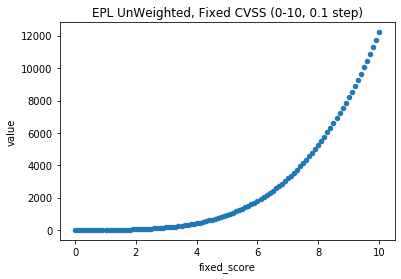
\includegraphics[width=\linewidth]{output_37_1.png} 
        \caption{Distribution of observed non-normalized EPL} 
        \label{fig:automation:results:epl_dist_unnorm}
    \end{subfigure}
    %       \begin{subfigure}[t]{0.3\textwidth}
    %     \centering
    %     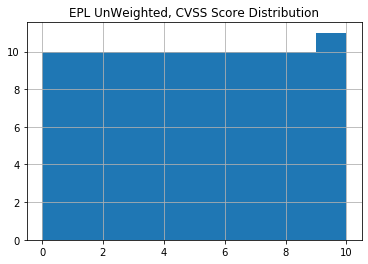
\includegraphics[width=\linewidth]{output_37_2.png}
    %     \caption{CVSS fixed uniformly}
    %     \label{fig:refnet_med}
    % \end{subfigure}
     \begin{subfigure}[t]{0.48\textwidth}
        \centering
        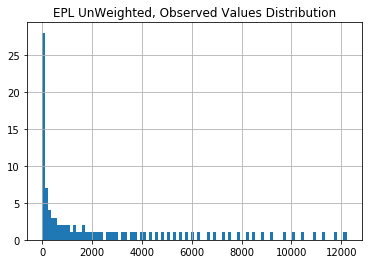
\includegraphics[width=\linewidth]{output_37_3.png}
        \caption{Exponential Distribution of EPL scores without normalization}
        \label{fig:automation:results:epl_scores_unnorm}
    \end{subfigure}
    \hfill
    \caption{Non-Normalized CVSS-weighted EPL (0-10, 0.1steps)}
    \label{fig:automation:results:epl_unnorm}
\end{figure}
\begin{figure}
    \centering
    \begin{subfigure}[t]{0.48\textwidth}
        % \centering
        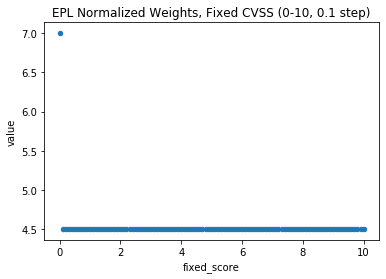
\includegraphics[width=\linewidth]{output_31_1.png} 
        \caption{Normalizing counters the effect of CVSS scoring} 
        \label{fig:automation:results:epl_scores_norm}
    \end{subfigure}
    %       \begin{subfigure}[t]{0.3\textwidth}
    %     \centering
    %     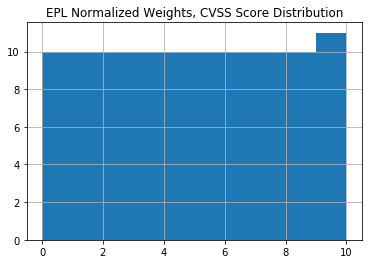
\includegraphics[width=\linewidth]{output_31_2.png}
    %     \caption{CVSS fixed uniformly}
    %     \label{fig:refnet_med}
    % \end{subfigure}
     \begin{subfigure}[t]{0.48\textwidth}
        \centering
        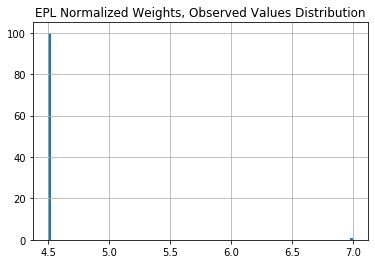
\includegraphics[width=\linewidth]{output_31_3.png}
        \caption{All observed values nearly identical}
        \label{fig:automation:results:epl_dist_norm}
    \end{subfigure}
    \hfill
    \caption{Normalized CVSS-weighted EPL (0-10, 0.1steps) }
    \label{fig:automation:results:epl_norm}
\end{figure}

% \begin{figure}
%     \centering
%     \begin{subfigure}[t]{0.48\textwidth}
%         % \centering
%         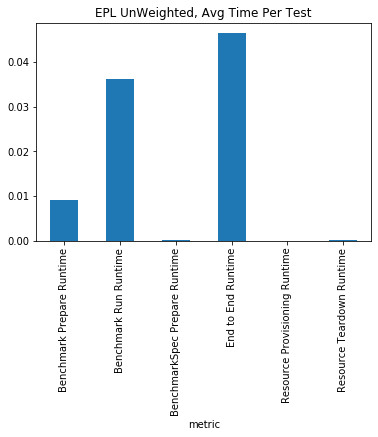
\includegraphics[width=\linewidth]{output_44_0.png} 
%         \caption{Unnormalized EPL times} 
%         \label{fig:automation:results:unnorm_epl_times}
%     \end{subfigure}
%           \begin{subfigure}[t]{0.48\textwidth}
%         \centering
%         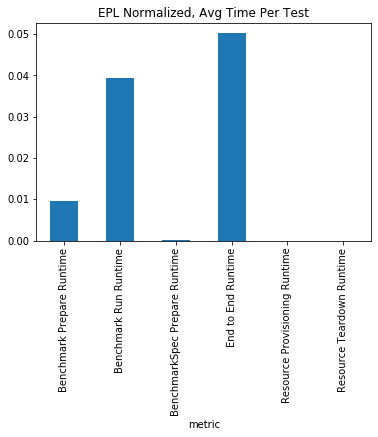
\includegraphics[width=\linewidth]{output_47_0.png}
%         \caption{Normalized EPL times}
%         \label{fig:automation:results:norm_epl_timings}
%     \end{subfigure}
%         \hfill
%     \caption{Mean time in each pipeline stage}\label{fig:automation:results:timings}
% \end{figure}

In Figure \ref{fig:mttf_score_distributions} we fix the vulnerability placement of two different input models representing a \textit{small} and \textit{large} enterprises, and select CVSS scores from a uniform random distribution. We create 1000 samples in this manner and observe the distribution and kernel density estimates of MTTF\cite{Dacier_Deswarte_Kaaniche} scores for all samples. Note that Dacier uses the arrival rates shown in Listing \ref{lst:map_mttf} to estimate the time an attacker would need to compromise each vulnerability, and we map the randomly assigned CVSS scores to these arrival rates at uniform intervals. The accumulation points observed in the small network occur at seemingly discrete boundaries (x-axis is shown in weeks, where 0 is approximately instantaneous compromise), while the large network demonstrates a more compressed time to compromise over all observed samples, with nearly all vulnerability score distribution resulting in nearly immediate compromise. This distribution of observed MTTF scores is confirmed in Figure \ref{fig:score_map_stepping} where we maintain the same input models and vulnerability placement as shown in Figure \ref{fig:mttf_score_distributions}, but fix all CVSS scores in the range 0.0-10.0 increasing the score by 0.1 for each sample. The resulting step-wise graph shows the boundary of each mapping interval used, but more importantly, we can clearly observe the range of values in the small network is between 0 and 200 weeks, while the range of the larger network is restricted between 0 and 50 weeks. This discrepancy in achievable MTTF scores means that the size of the network impacts the range of values observed, which should be understood before selecting this measurement for use in operational environments.

In Figures \ref{fig:automation:results:epl_norm} and \ref{fig:automation:results:epl_unnorm} we demonstrate the impact of normalization on security measurement values using a procedure similar to that above. In this case we observe the Expected Path Length\cite{Abraham_Nair_2014}  metric over fixed CVSS scores in the range 0.0-10.0 incrementing again by 0.1 for each sample. In Figure \ref{fig:automation:results:epl_unnorm} we refrain from normalizing the scores used in EPL calculation and observe an exponential increase in observed values from 0 to around 12000 days as all vulnerability scores are raised from 0.0 (easily exploited) to 10 (most difficult to exploit). In Figure  \ref{fig:automation:results:epl_norm} we run the same experiment, although this time with the following normalization method to determine the transition probability: $p(i,j)=\frac{e_j}{\sum_{k=1}^{n}e_k}$ where n is the number of outgoing edges from node $i$ and $e_j$ is the CVSS exploitability score for the vulnerability in state $j$. Our immediate observation is the this normalization effectively undermines the effect of CVSS weighting, as the range of EPL values remains nearly constant after performing this operation. We would also note here that there are several proposed security metrics in the literature that apply some type of normalization to their transition scores with the intent of creating stochastic models, and we are currently evaluating the effects of different scoring and weighting strategies to the behaviour of the underlying metrics. 

In figure \ref{fig:automation:results:timings} we demonstrate how our implementation can be used to profile metrics and capture performance related metrics of the security metrics under evaluation. Possibly of less concern than the behavioural analyses shown above, when we wish to compare security metric implementations which can be either analytical (for example, the authors propose matrix inversion in their calculation) or stochastic (where simulations are run to estimate the same metric) then we can not only use our framework to confirm both metrics converge on the same value, but also determine which metric does so more efficiently. We therefore enable capturing timings related to each step in the processing pipeline, from input modeling and transformation, to calculation and teardown.



% \begin{figure}
%     \centering
%     \begin{subfigure}[t]{1in}        
%         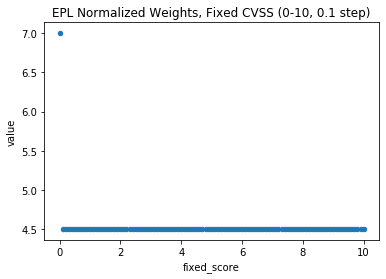
\includegraphics[width=1in]{output_31_1.png}     
%         \caption{}
%     \end{subfigure}    
    
%     \begin{subfigure}[t]{1in}        
%         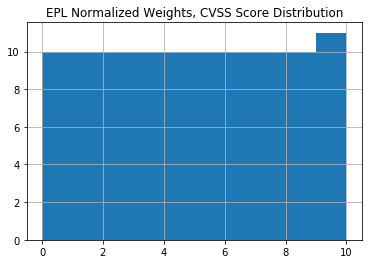
\includegraphics[width=1in]{output_31_2.png}  
%         \caption{}
%     \end{subfigure}
    
%     \medskip  % <-------------------------------  
    
%     \begin{subfigure}[t]{1.5in}
%         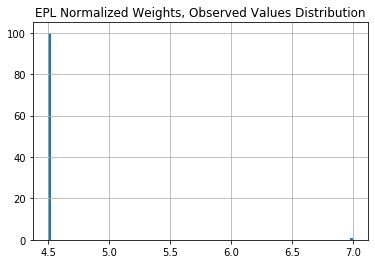
\includegraphics[width=1.5in]{output_31_3.png}
%         \caption{}
%     \end{subfigure}    
     
%      \begin{subfigure}[t]{1.5in}            
%         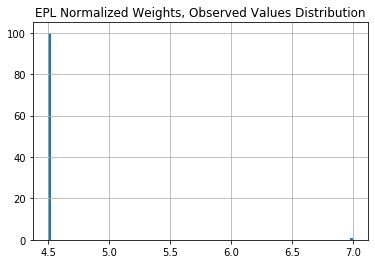
\includegraphics[width=1.5in]{output_31_3.png}   
%         \caption{}
%     \end{subfigure}
    
%     \medskip  % <------------------------------- 
    
%     \begin{subfigure}[t]{1.5in}
%         \centering
%         % \caption{Prelec}
%             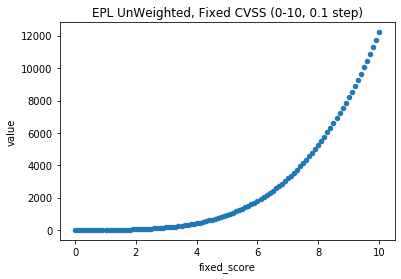
\includegraphics[width=1.5in]{output_37_1.png}  
%             \caption{}
%     \end{subfigure}
    
% %            \caption{Prelec}%\label{fig:2b}
%     \begin{subfigure}[t]{1.5in}
%         \centering
%                 % \caption{Prelec}
%         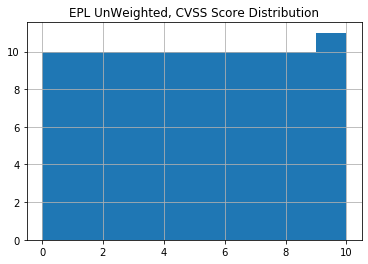
\includegraphics[width=1.5in]{output_37_2.png} 
%         \caption{}
%     \end{subfigure}
    
    
    
    
        
%     \centering
%     \caption{Classifier Error Plots (Predicted vs Actual) for the system's calculated security}\label{fig:ml:classifier_errors} 
% \end{figure}
